\documentclass{article}
\usepackage{fancyvrb}
\usepackage[utf8]{inputenc}
\usepackage{graphicx}
\usepackage{float}
\usepackage{pdfpages}
\graphicspath{{./img/}}
\usepackage[a4paper]{geometry}
\geometry{top=3cm, bottom=3.0cm, left=3cm, right=3.5cm}
\graphicspath{{./img/}}
\PassOptionsToPackage{hyphens}{url}
\usepackage{hyperref}


\begin{document}

\title{
	\textbf{Práctica 3: Desarrollo de una aplicación multiplataforma}
}
\author{Noelia Escalera Mejías - Jesús Torres Sánchez}
\maketitle

\section{Descripción}
Se ha decidido implementar una aplicación de votaciones conjuntas siguiendo un modelo cliente-servidor. Por un lado, tendremos una web encargada de recoger los resultados de la votación y mostrarlos posteriormente. Por otro lado tendremos una aplicación que se comunicará con la web y desde la cuál cada usuario introducirá sus votos.

\section{Requisitos funcionales}
\begin{itemize}
	\item \textbf{RF-1.} Alta de usuario.
	\item \textbf{RF-2.} Unirse a votación.
	\item \textbf{RF-3.} Crear una sala de votación.
	\item \textbf{RF-4.} Votar en una votación.
	\item \textbf{RF-5.} Consultar resultados.
	\item \textbf{RF-6.} Seleccionar tipo de votación. \\
\end{itemize}

\section{Requisitos no funcionales}
\begin{itemize}
	\item \textbf{RNF-1}. La interfaz gráfica será sencilla con el objetivo de facilitar el uso para la mayoría de usuarios.
	\item \textbf{RNF-2.} Al establecer comunicaciones con un servidor web debemos tener
	en cuenta múltiples aspectos de seguridad tanto en la propia aplicación
	como en el servidor en sí.
	\item \textbf{RNF-3}. La aplicación tiene que tener facilidad para ser portable.
	\item \textbf{RNF-4}. El servidor debe estar disponible en todo momento para poder
	acceder a las distintas votaciones en tiempo real.
	\item \textbf{RNF-5}. Habrá una amplia variedad de votaciones para elegir.
\end{itemize}

\section{Diagrama de clases de diseño}
A continuación se adjunta un diagrama de clases de diseño provisional, dónde se especifican los elementos más importantes del sistema así como las relaciones entre los mismos:

\begin{figure}[H]
	\centering
	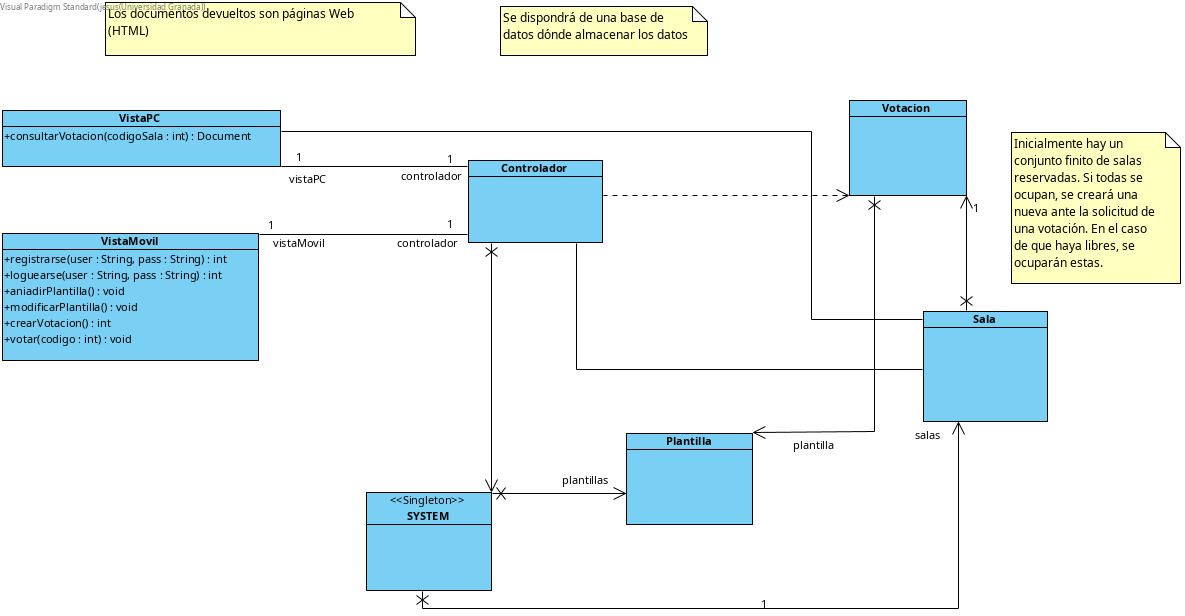
\includegraphics[totalheight=9.25cm]{img/diagrama_clases}
	\caption{Diagrama de clases de diseño}
	\label{fig:figura1}
\end{figure}

Este diagrama de clases está incompleto, ya que solamente contiene las operaciones de las vistas y no muestra la información almacenada, aunque nos sirve de ayuda para modelar inicialmente el sistema.

\section{Desarrollo de la aplicación}
En nuestro caso, la aplicación dispondrá de una interfaz web y otra móvil, cada una proporcionando las operaciones mostradas en el diagrama de clases anterior. \\
Por ahora, solamente hemos desarrollado una versión inicial del servidor web, incluyendo todas las operaciones (tanto las de la interfaz móvil como las de la web) dentro de una interfaz web uniforme. Para ello, hemos decidido usar Node.js ya que se adecúa perfectamente a los requerimientos de nuestra aplicación. \\ ~ \\
Esta interfaz es completamente primitiva: no dispone de ninguna hoja de estilos para mostrar la información de forma amigable al usuario ni incluye la gestión de usuarios. El funcionamiento de esta versión es el siguiente:
\begin{itemize}
	\item Al acceder al servidor, indicamos el código de la sala y la operación a realizar (votar o consultar). En la versión final, la interfaz web solamente incluirá la opción de consultar, aunque en esta versión se ha incluido para entender mejor su funcionamiento.
	

	\item Inicialmente no hay ninguna votación creada (y por tanto ninguna sala reservada). Para crear las votaciones, partimos de una serie de plantillas prefabricadas: inicialmente no tenemos ninguna, por lo que se incluirá además la opción de crear una nueva plantilla que se podrá usar en la creación de una votación. Para ello, accederemos concatenando a la url la cadena \textit{new-template}.
	
	\begin{figure}[H]
		\centering
		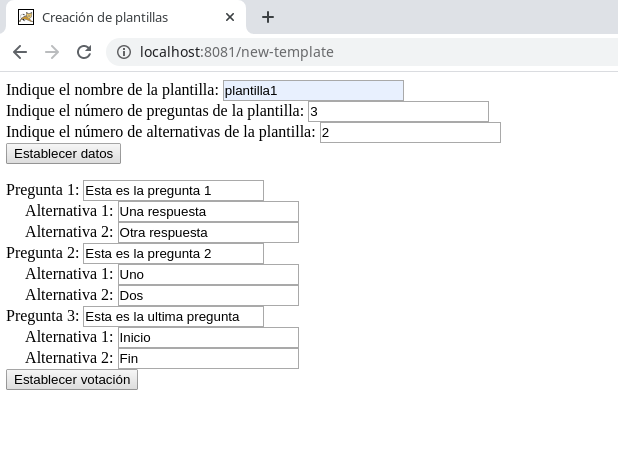
\includegraphics[totalheight=9.25cm]{img/cap1}
		\caption{Captura 1}
		\label{fig:figura2}
	\end{figure}

	\item Una vez tenemos creada la plantilla, creamos una nueva votación. Para acceder al formulario de creación de una votación se concatenará a la url la cadena \textit{new-voting}. En este caso, una vez hayamos seleccionado la plantilla, el servidor gestionará la petición y devolverá un código de sala.
	
	\begin{figure}[H]
		\centering
		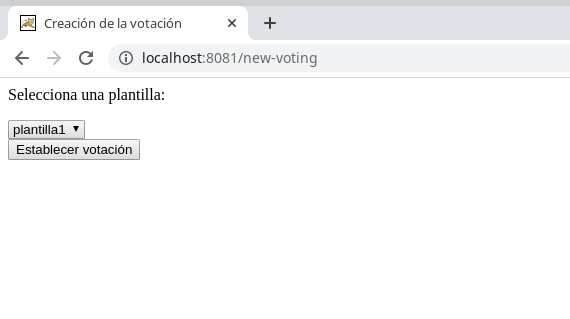
\includegraphics[totalheight=6.25cm]{img/cap2}
		\caption{Captura 2}
		\label{fig:figura3}
	\end{figure}

	\begin{figure}[H]
		\centering
		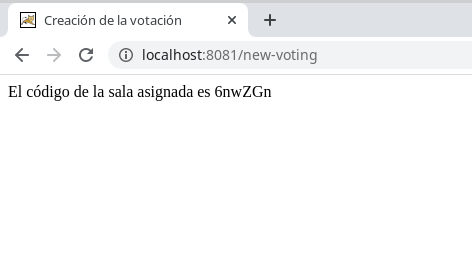
\includegraphics[totalheight=5.25cm]{img/cap3}
		\caption{Captura 3}
		\label{fig:figura4}
	\end{figure}

	\item Finalmente, conforme se vayan realizando los votos a las alternativas de las distintas preguntas, la información se actualiza en tiempo real en todos los navegadores. 
	
	\begin{figure}[H]
		\centering
		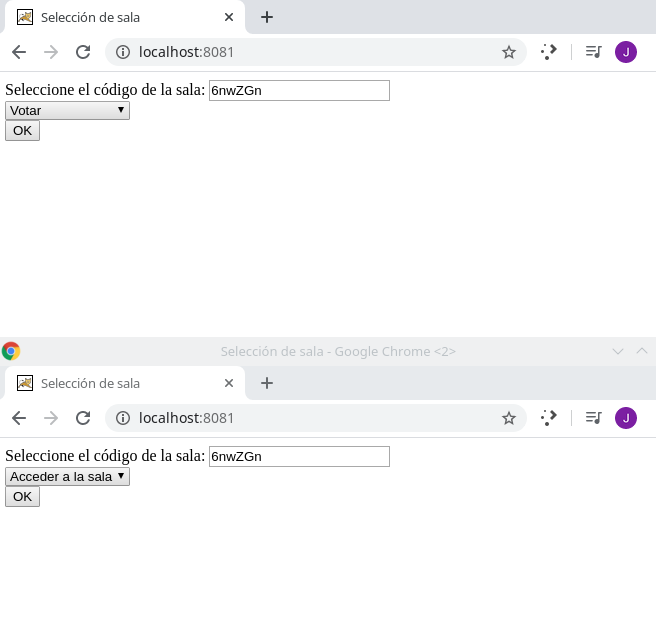
\includegraphics[totalheight=10.25cm]{img/cap4}
		\caption{Captura 4}
		\label{fig:figura5}
	\end{figure}

	\begin{figure}[H]
		\centering
		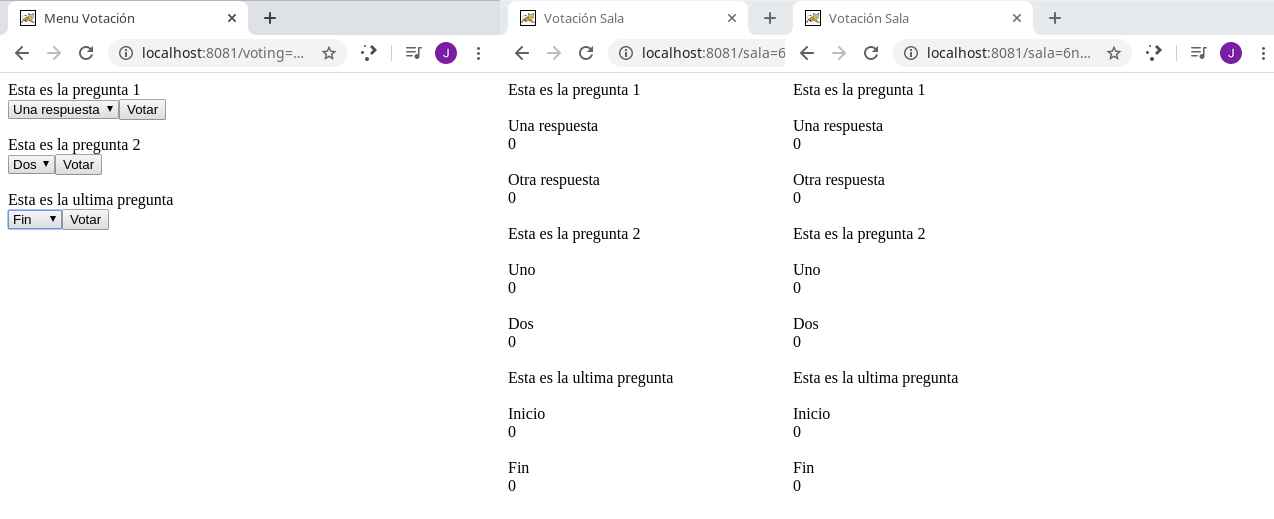
\includegraphics[totalheight=9cm]{img/cap5}
		\caption{Captura 5}
		\label{fig:figura6}
	\end{figure}

	\begin{figure}[H]
		\centering
		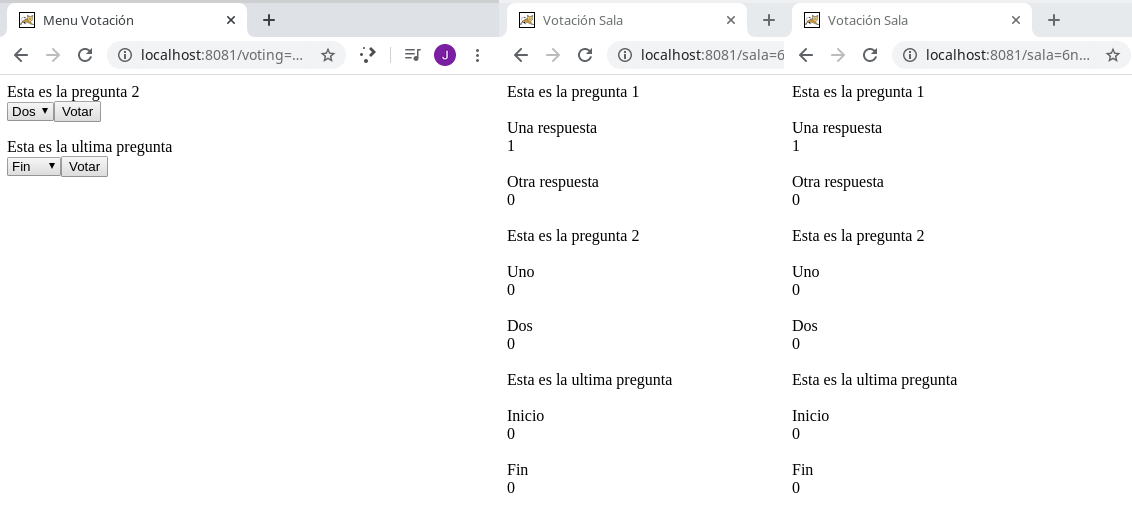
\includegraphics[totalheight=9cm]{img/cap6}
		\caption{Captura 6}
		\label{fig:figura7}
	\end{figure}

	\begin{figure}[H]
		\centering
		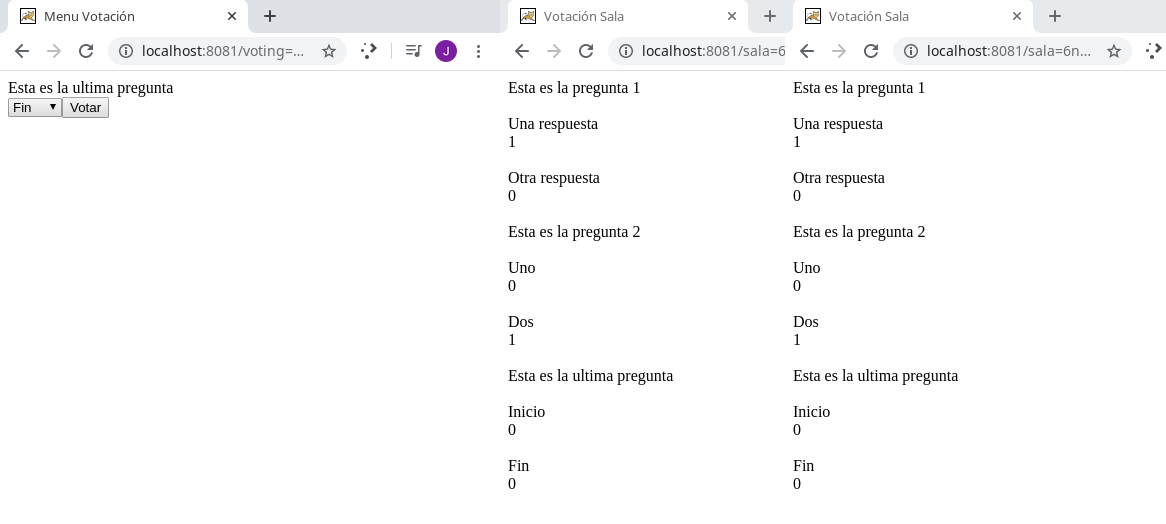
\includegraphics[totalheight=9cm]{img/cap7}
		\caption{Captura 7}
		\label{fig:figura8}
	\end{figure}

	\begin{figure}[H]
		\centering
		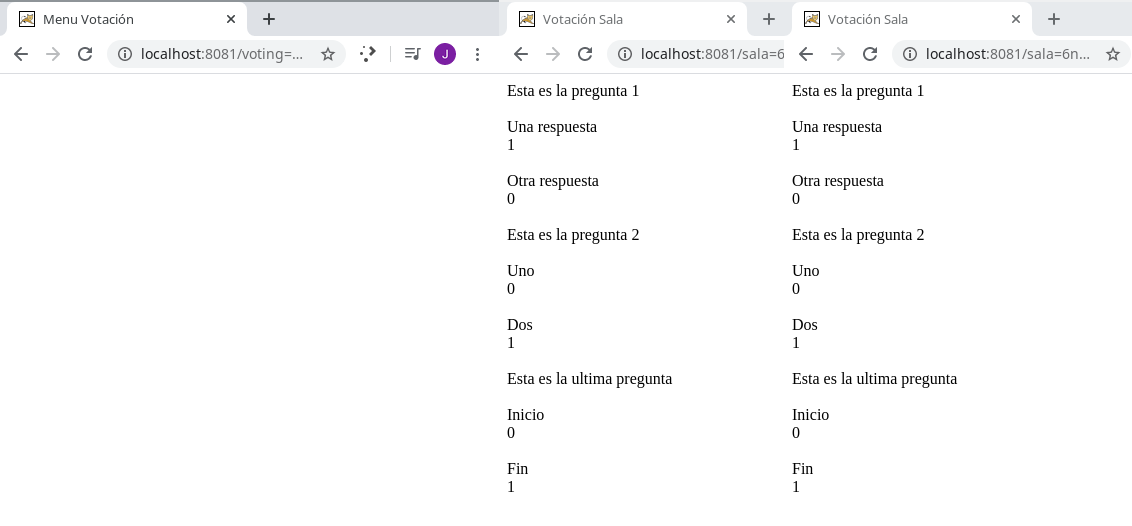
\includegraphics[totalheight=9cm]{img/cap8}
		\caption{Captura 8}
		\label{fig:figura9}
	\end{figure}
\end{itemize}
\end{document}